% Options for packages loaded elsewhere
\PassOptionsToPackage{unicode}{hyperref}
\PassOptionsToPackage{hyphens}{url}
%
\documentclass[
]{article}
\usepackage{lmodern}
\usepackage{amssymb,amsmath}
\usepackage{ifxetex,ifluatex}
\ifnum 0\ifxetex 1\fi\ifluatex 1\fi=0 % if pdftex
  \usepackage[T1]{fontenc}
  \usepackage[utf8]{inputenc}
  \usepackage{textcomp} % provide euro and other symbols
\else % if luatex or xetex
  \usepackage{unicode-math}
  \defaultfontfeatures{Scale=MatchLowercase}
  \defaultfontfeatures[\rmfamily]{Ligatures=TeX,Scale=1}
\fi
% Use upquote if available, for straight quotes in verbatim environments
\IfFileExists{upquote.sty}{\usepackage{upquote}}{}
\IfFileExists{microtype.sty}{% use microtype if available
  \usepackage[]{microtype}
  \UseMicrotypeSet[protrusion]{basicmath} % disable protrusion for tt fonts
}{}
\makeatletter
\@ifundefined{KOMAClassName}{% if non-KOMA class
  \IfFileExists{parskip.sty}{%
    \usepackage{parskip}
  }{% else
    \setlength{\parindent}{0pt}
    \setlength{\parskip}{6pt plus 2pt minus 1pt}}
}{% if KOMA class
  \KOMAoptions{parskip=half}}
\makeatother
\usepackage{xcolor}
\IfFileExists{xurl.sty}{\usepackage{xurl}}{} % add URL line breaks if available
\IfFileExists{bookmark.sty}{\usepackage{bookmark}}{\usepackage{hyperref}}
\hypersetup{
  pdftitle={Intro to R (Honors Seminar 2020)},
  pdfauthor={Elena Barham},
  hidelinks,
  pdfcreator={LaTeX via pandoc}}
\urlstyle{same} % disable monospaced font for URLs
\usepackage[margin=1in]{geometry}
\usepackage{color}
\usepackage{fancyvrb}
\newcommand{\VerbBar}{|}
\newcommand{\VERB}{\Verb[commandchars=\\\{\}]}
\DefineVerbatimEnvironment{Highlighting}{Verbatim}{commandchars=\\\{\}}
% Add ',fontsize=\small' for more characters per line
\usepackage{framed}
\definecolor{shadecolor}{RGB}{248,248,248}
\newenvironment{Shaded}{\begin{snugshade}}{\end{snugshade}}
\newcommand{\AlertTok}[1]{\textcolor[rgb]{0.94,0.16,0.16}{#1}}
\newcommand{\AnnotationTok}[1]{\textcolor[rgb]{0.56,0.35,0.01}{\textbf{\textit{#1}}}}
\newcommand{\AttributeTok}[1]{\textcolor[rgb]{0.77,0.63,0.00}{#1}}
\newcommand{\BaseNTok}[1]{\textcolor[rgb]{0.00,0.00,0.81}{#1}}
\newcommand{\BuiltInTok}[1]{#1}
\newcommand{\CharTok}[1]{\textcolor[rgb]{0.31,0.60,0.02}{#1}}
\newcommand{\CommentTok}[1]{\textcolor[rgb]{0.56,0.35,0.01}{\textit{#1}}}
\newcommand{\CommentVarTok}[1]{\textcolor[rgb]{0.56,0.35,0.01}{\textbf{\textit{#1}}}}
\newcommand{\ConstantTok}[1]{\textcolor[rgb]{0.00,0.00,0.00}{#1}}
\newcommand{\ControlFlowTok}[1]{\textcolor[rgb]{0.13,0.29,0.53}{\textbf{#1}}}
\newcommand{\DataTypeTok}[1]{\textcolor[rgb]{0.13,0.29,0.53}{#1}}
\newcommand{\DecValTok}[1]{\textcolor[rgb]{0.00,0.00,0.81}{#1}}
\newcommand{\DocumentationTok}[1]{\textcolor[rgb]{0.56,0.35,0.01}{\textbf{\textit{#1}}}}
\newcommand{\ErrorTok}[1]{\textcolor[rgb]{0.64,0.00,0.00}{\textbf{#1}}}
\newcommand{\ExtensionTok}[1]{#1}
\newcommand{\FloatTok}[1]{\textcolor[rgb]{0.00,0.00,0.81}{#1}}
\newcommand{\FunctionTok}[1]{\textcolor[rgb]{0.00,0.00,0.00}{#1}}
\newcommand{\ImportTok}[1]{#1}
\newcommand{\InformationTok}[1]{\textcolor[rgb]{0.56,0.35,0.01}{\textbf{\textit{#1}}}}
\newcommand{\KeywordTok}[1]{\textcolor[rgb]{0.13,0.29,0.53}{\textbf{#1}}}
\newcommand{\NormalTok}[1]{#1}
\newcommand{\OperatorTok}[1]{\textcolor[rgb]{0.81,0.36,0.00}{\textbf{#1}}}
\newcommand{\OtherTok}[1]{\textcolor[rgb]{0.56,0.35,0.01}{#1}}
\newcommand{\PreprocessorTok}[1]{\textcolor[rgb]{0.56,0.35,0.01}{\textit{#1}}}
\newcommand{\RegionMarkerTok}[1]{#1}
\newcommand{\SpecialCharTok}[1]{\textcolor[rgb]{0.00,0.00,0.00}{#1}}
\newcommand{\SpecialStringTok}[1]{\textcolor[rgb]{0.31,0.60,0.02}{#1}}
\newcommand{\StringTok}[1]{\textcolor[rgb]{0.31,0.60,0.02}{#1}}
\newcommand{\VariableTok}[1]{\textcolor[rgb]{0.00,0.00,0.00}{#1}}
\newcommand{\VerbatimStringTok}[1]{\textcolor[rgb]{0.31,0.60,0.02}{#1}}
\newcommand{\WarningTok}[1]{\textcolor[rgb]{0.56,0.35,0.01}{\textbf{\textit{#1}}}}
\usepackage{longtable,booktabs}
% Correct order of tables after \paragraph or \subparagraph
\usepackage{etoolbox}
\makeatletter
\patchcmd\longtable{\par}{\if@noskipsec\mbox{}\fi\par}{}{}
\makeatother
% Allow footnotes in longtable head/foot
\IfFileExists{footnotehyper.sty}{\usepackage{footnotehyper}}{\usepackage{footnote}}
\makesavenoteenv{longtable}
\usepackage{graphicx,grffile}
\makeatletter
\def\maxwidth{\ifdim\Gin@nat@width>\linewidth\linewidth\else\Gin@nat@width\fi}
\def\maxheight{\ifdim\Gin@nat@height>\textheight\textheight\else\Gin@nat@height\fi}
\makeatother
% Scale images if necessary, so that they will not overflow the page
% margins by default, and it is still possible to overwrite the defaults
% using explicit options in \includegraphics[width, height, ...]{}
\setkeys{Gin}{width=\maxwidth,height=\maxheight,keepaspectratio}
% Set default figure placement to htbp
\makeatletter
\def\fps@figure{htbp}
\makeatother
\setlength{\emergencystretch}{3em} % prevent overfull lines
\providecommand{\tightlist}{%
  \setlength{\itemsep}{0pt}\setlength{\parskip}{0pt}}
\setcounter{secnumdepth}{5}

\title{Intro to R (Honors Seminar 2020)}
\author{Elena Barham}
\date{9/30/2020}

\begin{document}
\maketitle

\hypertarget{load-packages}{%
\section{Load Packages}\label{load-packages}}

\begin{Shaded}
\begin{Highlighting}[]
\CommentTok{### General use packages }
\CommentTok{# tidyverse # This package is actually a suite of packages }
\CommentTok{# raster    # Reading, writing, and manipulating raster form spatial data }
\CommentTok{# rgdal     # Provides access to spatial projection operations }
\CommentTok{# GISTools  # Choropleth plots and aggregation of point data to polygons }
\CommentTok{# rgeos     # Operations with spatial data (i.e. intersection, length of spatial forms)}
\CommentTok{# maptools  # More tools for manipulating geographic data }
\CommentTok{# ggplot2   # for graphing}

\CommentTok{# A function to see if we need to load}
\NormalTok{check.packages <-}\StringTok{ }\ControlFlowTok{function}\NormalTok{(pkg)\{}
\NormalTok{  new.pkg <-}\StringTok{ }\NormalTok{pkg[}\OperatorTok{!}\NormalTok{(pkg }\OperatorTok\StringTok{ }\KeywordTok{installed.packages}\NormalTok{()[, }\StringTok{"Package"}\NormalTok{])]}
  \ControlFlowTok{if}\NormalTok{ (}\KeywordTok{length}\NormalTok{(new.pkg))}
    \KeywordTok{install.packages}\NormalTok{(new.pkg, }\DataTypeTok{dependencies =} \OtherTok{TRUE}\NormalTok{,}
                     \DataTypeTok{repos =} \StringTok{"https://cran.rstudio.com"}\NormalTok{)}
  \KeywordTok{sapply}\NormalTok{(pkg, require, }\DataTypeTok{character.only =} \OtherTok{TRUE}\NormalTok{)}
\NormalTok{\}}

\NormalTok{pkgList <-}\StringTok{ }
\StringTok{  }\KeywordTok{c}\NormalTok{(}\StringTok{"raster"}\NormalTok{, }\StringTok{"rgdal"}\NormalTok{, }\StringTok{"GISTools"}\NormalTok{, }\StringTok{"rgeos"}\NormalTok{, }
    \StringTok{"maptools"}\NormalTok{, }\StringTok{"ggplot2"}\NormalTok{, }\StringTok{"haven"}\NormalTok{, }\StringTok{"stargazer"}\NormalTok{, }\StringTok{"sp"}\NormalTok{, }\StringTok{"knitr"}\NormalTok{)}

\KeywordTok{check.packages}\NormalTok{(pkgList)}
\end{Highlighting}
\end{Shaded}

\begin{verbatim}
##    raster     rgdal  GISTools     rgeos  maptools   ggplot2     haven stargazer 
##      TRUE      TRUE      TRUE      TRUE      TRUE      TRUE      TRUE      TRUE 
##        sp     knitr 
##      TRUE      TRUE
\end{verbatim}

Note that you first need to install packages and then save them to your
library. Once you have installed them once you then just need to add
them to the library for new sessions.

\hypertarget{learning-some-basic-commands}{%
\subsection{Learning Some Basic
Commands}\label{learning-some-basic-commands}}

\begin{Shaded}
\begin{Highlighting}[]
\NormalTok{x <-}\StringTok{ }\DecValTok{3} \CommentTok{#this assigns an object}
\NormalTok{x }\OperatorTok{==}\StringTok{ }\DecValTok{3} \CommentTok{#this is a logical question }
\end{Highlighting}
\end{Shaded}

\begin{verbatim}
## [1] TRUE
\end{verbatim}

\begin{Shaded}
\begin{Highlighting}[]
\NormalTok{y <-}\StringTok{ "ABC"} \CommentTok{#this assigns a character string }

\NormalTok{x <-}\StringTok{ }\KeywordTok{c}\NormalTok{(}\DecValTok{3}\NormalTok{,}\DecValTok{4}\NormalTok{,}\DecValTok{5}\NormalTok{,}\DecValTok{6}\NormalTok{) }\CommentTok{#this is a numeric vector}
\NormalTok{m <-}\StringTok{ }\KeywordTok{c}\NormalTok{(}\StringTok{"panda"}\NormalTok{, }\StringTok{"octopus"}\NormalTok{, }\StringTok{"squirrel"}\NormalTok{, }\StringTok{"moose"}\NormalTok{) }\CommentTok{#this is a character vector }

\NormalTok{panda <-}\StringTok{ }\KeywordTok{c}\NormalTok{(x,m) }\CommentTok{# this combines x and m into one vector}
\NormalTok{panda <-}\StringTok{ }\KeywordTok{rbind}\NormalTok{(x,m) }\CommentTok{# this binds x and m into a matrix by rows}
\NormalTok{panda <-}\StringTok{ }\KeywordTok{cbind}\NormalTok{(x,m) }\CommentTok{# this binds x and m into a matrix by columns }

\NormalTok{panda <-}\StringTok{ }\KeywordTok{as.data.frame}\NormalTok{(panda) }\CommentTok{# this makes y into a data frame }

\NormalTok{a <-}\StringTok{ }\NormalTok{panda[,}\DecValTok{1}\NormalTok{] }\CommentTok{# this subsets y into the first column }
\NormalTok{b <-}\StringTok{ }\NormalTok{panda[}\DecValTok{1}\NormalTok{,] }\CommentTok{# this subsets y into the first row }
\end{Highlighting}
\end{Shaded}

\hypertarget{loading-and-merging-data---panel}{%
\subsection{Loading and merging data -
PANEL}\label{loading-and-merging-data---panel}}

\begin{Shaded}
\begin{Highlighting}[]
\CommentTok{# Load panel data }
\NormalTok{mexico <-}\StringTok{ }\KeywordTok{read.csv}\NormalTok{(}\StringTok{"mexico.csv"}\NormalTok{)}

\CommentTok{# Make sure our data is there}
\CommentTok{#View(mexico)  # The 'View' function brings up the panel data}

\CommentTok{# Load a stata file}
\NormalTok{elections <-}\StringTok{ }\KeywordTok{read_dta}\NormalTok{(}\StringTok{"mex_elections.dta"}\NormalTok{)}
\CommentTok{# Citing this data: Blackman, Allen; Villalobos, Laura, 2020, "Replication data for Use Forests or Lose Them? Regulated Timber Extraction and Tree Cover Loss in Mexico", https://doi.org/10.7910/DVN/NPUCWT, Harvard Dataverse, V1, UNF:6:ziy566ZTxSlzbBPEvBz+Nw== [fileUNF]}

\CommentTok{### Merging }\AlertTok{###}\CommentTok{   }
\CommentTok{# Merge two data frames - create a unique merge ID }


\CommentTok{#### Basic Cleaning Techniques }\AlertTok{###}\CommentTok{ }
\NormalTok{mexico}\OperatorTok{$}\NormalTok{X <-}\StringTok{ }\OtherTok{NULL} \CommentTok{# Delete extraneous columns  }
\NormalTok{mexico[}\KeywordTok{is.na}\NormalTok{(mexico}\OperatorTok{$}\NormalTok{GIS_AREA)] <-}\StringTok{ }\DecValTok{0} \CommentTok{# This sets NA observations of the variable attacks to '0' }
\NormalTok{mexico <-}\StringTok{ }\NormalTok{mexico[}\OperatorTok{!}\KeywordTok{is.na}\NormalTok{(mexico}\OperatorTok{$}\NormalTok{GOV_TYPE),] }\CommentTok{# This drops NA observations of the specified variable }

\CommentTok{## Merging }
\NormalTok{merged <-}\StringTok{ }\KeywordTok{merge}\NormalTok{(mexico, elections, }\DataTypeTok{by =} \StringTok{"estado"}\NormalTok{, }\DataTypeTok{all.x =} \OtherTok{TRUE}\NormalTok{)}
\end{Highlighting}
\end{Shaded}

\hypertarget{loading-and-merging-data-spatial}{%
\subsection{Loading and merging data --
Spatial}\label{loading-and-merging-data-spatial}}

\begin{Shaded}
\begin{Highlighting}[]
\CommentTok{# Load spatial data }
\NormalTok{mex_shp <-}\StringTok{ }\KeywordTok{readOGR}\NormalTok{(}\DataTypeTok{dsn =} \StringTok{"mex_shp"}\NormalTok{,}
                 \DataTypeTok{layer =} \StringTok{"MEX_adm2"}\NormalTok{) }
\end{Highlighting}
\end{Shaded}

\begin{verbatim}
## OGR data source with driver: ESRI Shapefile 
## Source: "C:\Dropbox\Teaching\Honors\2020-21\Honors_2021\1 Resources and Readings\Materials - Monday October 1\mex_shp", layer: "MEX_adm2"
## with 1853 features
## It has 11 fields
## Integer64 fields read as strings:  ID_0 ID_1 ID_2
\end{verbatim}

\begin{Shaded}
\begin{Highlighting}[]
\NormalTok{mex_pa_shp <-}\StringTok{  }\KeywordTok{readOGR}\NormalTok{(}\DataTypeTok{dsn =} \StringTok{"mex_PAs_shp"}\NormalTok{,}
                 \DataTypeTok{layer =} \StringTok{"areas"}\NormalTok{) }
\end{Highlighting}
\end{Shaded}

\begin{verbatim}
## OGR data source with driver: ESRI Shapefile 
## Source: "C:\Dropbox\Teaching\Honors\2020-21\Honors_2021\1 Resources and Readings\Materials - Monday October 1\mex_PAs_shp", layer: "areas"
## with 1196 features
## It has 36 fields
\end{verbatim}

\begin{Shaded}
\begin{Highlighting}[]
\CommentTok{# Subsetting Data }
\NormalTok{federal_PAs <-}\StringTok{ }\KeywordTok{subset}\NormalTok{(mex_pa_shp, gv_cl }\OperatorTok{==}\StringTok{ "federal"}\NormalTok{)}

\CommentTok{# Make sure our data is there }
\KeywordTok{plot}\NormalTok{(mex_shp) }\CommentTok{# The 'plot' function lets you look at version of the shape file with no attributes}
\end{Highlighting}
\end{Shaded}

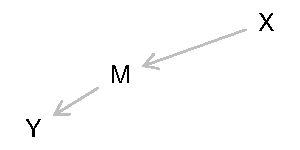
\includegraphics{Rmarkdown_forclass_2_files/figure-latex/unnamed-chunk-3-1.pdf}

\begin{Shaded}
\begin{Highlighting}[]
\KeywordTok{head}\NormalTok{(mex_shp, }\DecValTok{5}\NormalTok{) }\CommentTok{# The 'head' function lets you quickly look at the variables in a shape file }
\end{Highlighting}
\end{Shaded}

\begin{verbatim}
##   ID_0 ISO NAME_0 ID_1         NAME_1 ID_2         NAME_2    TYPE_2
## 0  145 MEX Mexico    1 Aguascalientes    1 Aguascalientes Municipio
## 1  145 MEX Mexico    1 Aguascalientes    2       Asientos Municipio
## 2  145 MEX Mexico    1 Aguascalientes    3       Calvillo Municipio
## 3  145 MEX Mexico    1 Aguascalientes    4         Cosío Municipio
## 4  145 MEX Mexico    1 Aguascalientes    5  Jesús María Municipio
##      ENGTYPE_2 NL_NAME_2   VARNAME_2
## 0 Municipality      <NA>        <NA>
## 1 Municipality      <NA>        <NA>
## 2 Municipality      <NA>        <NA>
## 3 Municipality      <NA>       Cosio
## 4 Municipality      <NA> Jesus Maria
\end{verbatim}

\hypertarget{data-exploration}{%
\subsection{Data Exploration}\label{data-exploration}}

\begin{verbatim}
     Min.   1st Qu.    Median      Mean   3rd Qu.      Max. 
  0.00146   0.19869   2.38153  19.09800  18.14911 199.52657 
\end{verbatim}

\begin{verbatim}

collaborative       federal         local     nonprofit       private 
            9           110            10             5           336 
  subnational 
          390 
\end{verbatim}

\begin{longtable}[]{@{}lrrrrrr@{}}
\toprule
& collaborative & federal & local & nonprofit & private &
subnational\tabularnewline
\midrule
\endhead
1954 & 0 & 1 & 0 & 0 & 0 & 0\tabularnewline
1959 & 0 & 1 & 0 & 0 & 0 & 0\tabularnewline
1962 & 0 & 1 & 0 & 0 & 0 & 0\tabularnewline
1964 & 0 & 1 & 0 & 0 & 0 & 0\tabularnewline
1972 & 0 & 0 & 0 & 0 & 0 & 2\tabularnewline
1975 & 0 & 0 & 0 & 0 & 0 & 1\tabularnewline
1976 & 0 & 0 & 0 & 0 & 0 & 1\tabularnewline
1977 & 0 & 0 & 0 & 0 & 0 & 7\tabularnewline
1978 & 0 & 0 & 0 & 0 & 0 & 5\tabularnewline
1979 & 0 & 0 & 0 & 0 & 0 & 2\tabularnewline
1980 & 0 & 1 & 0 & 0 & 0 & 4\tabularnewline
1981 & 0 & 4 & 0 & 0 & 0 & 2\tabularnewline
1982 & 0 & 2 & 0 & 0 & 0 & 1\tabularnewline
1983 & 0 & 0 & 0 & 0 & 0 & 1\tabularnewline
1986 & 0 & 0 & 0 & 0 & 0 & 2\tabularnewline
1987 & 0 & 1 & 0 & 0 & 0 & 2\tabularnewline
1988 & 0 & 3 & 0 & 0 & 0 & 3\tabularnewline
1989 & 0 & 0 & 0 & 0 & 0 & 1\tabularnewline
1990 & 0 & 0 & 0 & 0 & 0 & 2\tabularnewline
1991 & 0 & 1 & 0 & 0 & 0 & 3\tabularnewline
1992 & 0 & 3 & 0 & 0 & 0 & 5\tabularnewline
1993 & 0 & 0 & 0 & 0 & 0 & 8\tabularnewline
1994 & 0 & 4 & 0 & 0 & 0 & 8\tabularnewline
1995 & 0 & 1 & 0 & 0 & 0 & 37\tabularnewline
1996 & 0 & 1 & 0 & 0 & 0 & 45\tabularnewline
1997 & 0 & 2 & 0 & 0 & 0 & 11\tabularnewline
1998 & 0 & 5 & 0 & 0 & 0 & 8\tabularnewline
1999 & 0 & 1 & 0 & 0 & 0 & 9\tabularnewline
2000 & 0 & 15 & 0 & 0 & 0 & 28\tabularnewline
2001 & 0 & 2 & 0 & 0 & 0 & 8\tabularnewline
2002 & 0 & 20 & 0 & 0 & 1 & 11\tabularnewline
2003 & 0 & 3 & 0 & 0 & 1 & 15\tabularnewline
2004 & 2 & 3 & 0 & 2 & 5 & 29\tabularnewline
2005 & 1 & 5 & 1 & 1 & 5 & 20\tabularnewline
2006 & 0 & 1 & 0 & 1 & 43 & 25\tabularnewline
2007 & 0 & 2 & 0 & 0 & 15 & 19\tabularnewline
2008 & 4 & 8 & 7 & 1 & 9 & 16\tabularnewline
2009 & 0 & 5 & 1 & 0 & 14 & 14\tabularnewline
2010 & 0 & 4 & 0 & 0 & 53 & 13\tabularnewline
2011 & 1 & 1 & 0 & 0 & 58 & 6\tabularnewline
2012 & 0 & 4 & 0 & 0 & 35 & 3\tabularnewline
2013 & 1 & 2 & 1 & 0 & 19 & 4\tabularnewline
2014 & 0 & 0 & 0 & 0 & 18 & 3\tabularnewline
2015 & 0 & 1 & 0 & 0 & 9 & 2\tabularnewline
2016 & 0 & 0 & 0 & 0 & 8 & 4\tabularnewline
2017 & 0 & 1 & 0 & 0 & 26 & 0\tabularnewline
2018 & 0 & 0 & 0 & 0 & 11 & 0\tabularnewline
2019 & 0 & 0 & 0 & 0 & 6 & 0\tabularnewline
\bottomrule
\end{longtable}

\hypertarget{data-visualization---graphs}{%
\subsection{Data Visualization -
Graphs!}\label{data-visualization---graphs}}

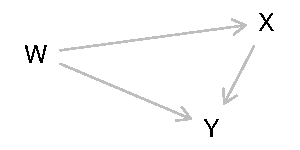
\includegraphics{Rmarkdown_forclass_2_files/figure-latex/unnamed-chunk-6-1.pdf}

\hypertarget{data-visualization---spatial}{%
\subsection{Data Visualization -
Spatial}\label{data-visualization---spatial}}

\begin{Shaded}
\begin{Highlighting}[]
\NormalTok{mex_shp <-}\StringTok{ }\KeywordTok{spTransform}\NormalTok{(mex_shp, }\KeywordTok{CRS}\NormalTok{(}\StringTok{"+proj=longlat +datum=WGS84 +no_defs"}\NormalTok{)) }\CommentTok{# Project }
\NormalTok{mex_pa_shp <-}\StringTok{ }\KeywordTok{spTransform}\NormalTok{(mex_pa_shp, }\KeywordTok{CRS}\NormalTok{(}\StringTok{"+proj=longlat +datum=WGS84 +no_defs"}\NormalTok{)) }\CommentTok{# Project }

\CommentTok{#Make a map! }
\KeywordTok{plot}\NormalTok{(mex_shp, }\DataTypeTok{col=}\StringTok{'light gray'}\NormalTok{, }\DataTypeTok{border=}\StringTok{'gray'}\NormalTok{)}
\KeywordTok{plot}\NormalTok{(}\KeywordTok{subset}\NormalTok{(mex_pa_shp, gv_cl }\OperatorTok{==}\StringTok{ "private"}\NormalTok{), }\DataTypeTok{add=}\OtherTok{TRUE}\NormalTok{, }\DataTypeTok{col=}\StringTok{"purple"}\NormalTok{, }\DataTypeTok{border =} \StringTok{"purple"}\NormalTok{)}
\end{Highlighting}
\end{Shaded}

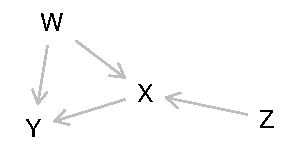
\includegraphics{Rmarkdown_forclass_2_files/figure-latex/unnamed-chunk-7-1.pdf}

\hypertarget{regression-and-displaying-results}{%
\subsection{Regression and Displaying
Results}\label{regression-and-displaying-results}}

\begin{Shaded}
\begin{Highlighting}[]
\CommentTok{# Basic Regression - these are nonsense specifications but }
\CommentTok{# will help you understand the form of how to specify a regression in r }
\NormalTok{x_}\DecValTok{1}\NormalTok{ <-}\StringTok{ }\KeywordTok{lm}\NormalTok{(federal }\OperatorTok{~}\StringTok{ }\NormalTok{participation, }\DataTypeTok{data =}\NormalTok{ merged)  }
\CommentTok{# summary(x_1)}

\CommentTok{# Fixed Effects }
\NormalTok{x_}\DecValTok{2}\NormalTok{ <-}\StringTok{ }\KeywordTok{lm}\NormalTok{(federal }\OperatorTok{~}\StringTok{ }\NormalTok{participation }\OperatorTok{+}\StringTok{ }\KeywordTok{as.factor}\NormalTok{(STATUS_YR), }\DataTypeTok{data =}\NormalTok{ merged)}
\CommentTok{# summary(x_2)}

\CommentTok{# Interaction Effects }
\NormalTok{x_}\DecValTok{3}\NormalTok{ <-}\StringTok{ }\KeywordTok{lm}\NormalTok{(federal }\OperatorTok{~}\StringTok{ }\NormalTok{participation}\OperatorTok{*}\NormalTok{povertyt1 }\OperatorTok{+}\StringTok{ }\KeywordTok{as.factor}\NormalTok{(STATUS_YR), }\DataTypeTok{data =}\NormalTok{ merged)}


\KeywordTok{stargazer}\NormalTok{(x_}\DecValTok{1}\NormalTok{, x_}\DecValTok{2}\NormalTok{, x_}\DecValTok{3}\NormalTok{, }\DataTypeTok{omit =} \StringTok{"STATUS_YR"}\NormalTok{, }
          \DataTypeTok{add.lines =} \KeywordTok{list}\NormalTok{(}\KeywordTok{c}\NormalTok{(}\StringTok{"Fixed effects?"}\NormalTok{, }\StringTok{"No"}\NormalTok{, }\StringTok{"Yes"}\NormalTok{, }\StringTok{"Yes"}\NormalTok{)),}
          \DataTypeTok{header=}\OtherTok{FALSE}\NormalTok{) }\CommentTok{# This produces a table that can be typeset in LaTeX. }
\end{Highlighting}
\end{Shaded}

\begin{table}[!htbp] \centering 
  \caption{} 
  \label{} 
\begin{tabular}{@{\extracolsep{5pt}}lccc} 
\\[-1.8ex]\hline 
\hline \\[-1.8ex] 
 & \multicolumn{3}{c}{\textit{Dependent variable:}} \\ 
\cline{2-4} 
\\[-1.8ex] & \multicolumn{3}{c}{federal} \\ 
\\[-1.8ex] & (1) & (2) & (3)\\ 
\hline \\[-1.8ex] 
 participation & $-$0.003$^{*}$ & $-$0.0003 & $-$0.018$^{***}$ \\ 
  & (0.002) & (0.002) & (0.006) \\ 
  & & & \\ 
 povertyt1 &  &  & $-$0.033$^{***}$ \\ 
  &  &  & (0.008) \\ 
  & & & \\ 
 participation:povertyt1 &  &  & 0.0005$^{***}$ \\ 
  &  &  & (0.0001) \\ 
  & & & \\ 
 Constant & 0.281$^{***}$ & 1.016$^{***}$ & 2.228$^{***}$ \\ 
  & (0.093) & (0.290) & (0.418) \\ 
  & & & \\ 
\hline \\[-1.8ex] 
Fixed effects? & No & Yes & Yes \\ 
Observations & 746 & 746 & 746 \\ 
R$^{2}$ & 0.004 & 0.337 & 0.370 \\ 
Adjusted R$^{2}$ & 0.003 & 0.293 & 0.325 \\ 
Residual Std. Error & 0.324 (df = 744) & 0.273 (df = 698) & 0.266 (df = 696) \\ 
F Statistic & 3.072$^{*}$ (df = 1; 744) & 7.555$^{***}$ (df = 47; 698) & 8.335$^{***}$ (df = 49; 696) \\ 
\hline 
\hline \\[-1.8ex] 
\textit{Note:}  & \multicolumn{3}{r}{$^{*}$p$<$0.1; $^{**}$p$<$0.05; $^{***}$p$<$0.01} \\ 
\end{tabular} 
\end{table}

\end{document}
